%% Преамбула TeX-файла

% 1. Стиль и язык
\documentclass[utf8x, 14pt]{G7-32} % Стиль (по умолчанию будет 14pt)

\usepackage{totcount}
\usepackage{listings}
\lstset{basicstyle=\footnotesize\ttfamily}
\lstset{frame=bottomline. frame=topline}

\newtotcounter{citnum} %From the package documentation
\def\oldbibitem{} \let\oldbibitem=\bibitem
\def\bibitem{\stepcounter{citnum}\oldbibitem}

\usepackage{etoolbox}

\newcounter{totfigures}

\providecommand\totfig{}

\makeatletter
\AtEndDocument{%
  \addtocounter{totfigures}{\value{figure}}%
  \immediate\write\@mainaux{%
    \string\gdef\string\totfig{\number\value{totfigures}}%
  }%
}
\makeatother

\pretocmd{\chapter}{\addtocounter{totfigures}{\value{figure}}\setcounter{figure}{0}}{}{}


% Остальные стандартные настройки убраны в preamble.inc.tex.
\sloppy

% Настройки стиля ГОСТ 7-32
% Для начала определяем, хотим мы или нет, чтобы рисунки и таблицы нумеровались в пределах раздела, или нам нужна сквозная нумерация.
\EqInChapter % формулы будут нумероваться в пределах раздела
\TableInChapter % таблицы будут нумероваться в пределах раздела
\PicInChapter % рисунки будут нумероваться в пределах раздела

% Добавляем гипертекстовое оглавление в PDF
\usepackage[
bookmarks=true, colorlinks=true, unicode=true,
urlcolor=black,linkcolor=black, anchorcolor=black,
citecolor=black, menucolor=black, filecolor=black,
]{hyperref}

% Изменение начертания шрифта --- после чего выглядит таймсоподобно.
% apt-get install scalable-cyrfonts-tex

\IfFileExists{cyrtimes.sty}
    {
        \usepackage{cyrtimespatched}
    }
    {
        % А если Times нету, то будет CM...
    }

\usepackage{graphicx}   % Пакет для включения рисунков
\DeclareGraphicsExtensions{.jpg,.pdf,.png}
% С такими оно полями оно работает по-умолчанию:
% \RequirePackage[left=20mm,right=10mm,top=20mm,bottom=20mm,headsep=0pt]{geometry}
% Если вас тошнит от поля в 10мм --- увеличивайте до 20-ти, ну и про переплёт не забывайте:
\geometry{right=20mm}
\geometry{left=30mm}



% Произвольная нумерация списков.
\usepackage{enumerate}
\usepackage{enumitem}
\usepackage{amsmath}
\usepackage{float}
\usepackage{subcaption}
\usepackage{listings}
\usepackage{lastpage}
\pagestyle{myheadings}
\DeclareMathOperator*{\argmax}{arg\,max}
\DeclareMathOperator*{\argmin}{arg\,min}

\setcounter{tocdepth}{1} %Подробность оглавления
%4 это chapter, section, subsection, subsubsection и paragraph
%3 это chapter, section, subsection и subsubsection
%2 это chapter, section, и subsection
%1 это chapter и section
%0 это chapter.

\setcounter{page}{2}

\begin{document}

\frontmatter % выключает нумерацию ВСЕГО; здесь начинаются ненумерованные главы: реферат, введение, глоссарий, сокращения и прочее.
\begin{center}
РЕФЕРАТ
\end{center}

% \large Московский авиационный институт\\[5.5cm]

% \huge Реферат \\[0.6cm] % название работы, затем отступ 0,6см
% \large на тему:  <<Метод идентификации музыкальных
% произведений по аудио фрагментам концертных исполнений>>\\[3.7cm]


% \end{center}

% \begin{flushright}
% Выполнил: студент гр. М8О-406Б \\
% Давид Гринберг \\
% \end{flushright}


% \vfill

% \begin{center}
% \large Москва 2020
% \end{center}

% \thispagestyle{empty}
Выпускная квалификационная работа содержит 43 страницы, \linebreak 15 рисунков, 3 таблицы, 7 листингов, 13 использованных источников.


КВАНТИЗАЦИЯ, МАШИННОЕ ОБУЧЕНИЕ, НЕЙРОННЫЕ СЕТИ, ОПТИМИЗАЦИЯ РАБОТЫ НЕЙРОСЕТЕЙ, C++, ЭФФЕКТИВНОЕ ПЕРЕМНОЖЕНИЕ МАТРИЦ, НИЗКОБИТОВЫЕ ВЫЧИСЛЕНИЯ, ОГРАНИЧЕННОСТЬ РЕСУРСОВ, ПРОМЕЖУТОЧНОЕ ГРАФОВОЕ ПРЕДСТАВЛЕНИЕ.

В данной работе реализуется квантизатор для перевода нейронных сетей в сжатый бинарный формат, в котором работа квантизованных слоёв реализовывается при помощи эффективного алгоритма перемножения матриц, основанного на работе побитовых операций.

В теоретической части работы приводится описание и математическое обоснование метода квантизации. Рассматривается и выводится алгоритм эффективного матричного произведения. Обосновывается формат хранения данных с точки зрения архитектуры современных процессоров. 

В практической части описывается процесс поддержки нового квантизованного слоя в рамках нейросетевого фреймворка Samsung ONE, включая сериализацию  и десериализацию параметров операции, поддержку слоя в промежуточном графовом представлении и создание вычислительного ядра в рамках интерпретатора нейросетевых моделей. Приводится анализ показателей квантизованного слоя в сравнении с исходной обученной глубокой моделью.

\setcounter{tocdepth}{4}
\setcounter{secnumdepth}{2}
\tableofcontents
\clearpage


\Introduction

\begin{center}
ВВЕДЕНИЕ
\end{center}

Нейронные  сети - мощный и современный инструмент для решения огромного множества задач, начиная от предсказания цен на недвижимость, основываясь на имеющихся характеристиках жилья, заканчивая генерацией или обработкой изображений в задачах компьютерного зрения. Нейронные сети сегодня используются повсюду, мы сталкиваемся с результатами их работы буквально каждый день. Однако возможность их применения ограничивается их ресурсоёмкостью: современные модели имеют миллионы настраиваемых параметров, что накладывает свой отпечаток не только на процесс обучения сети, ведь для обучения одной state-of-the-art нейронной модели необходимо иметь дорогостоящую ЭВМ или даже целый кластер, связанный в единую вычислительную систему, потратить огромное количество времени и электричества на каждую из попыток запуска алгоритма обучения при фиксированном наборе гиперпараметров, но и на использование уже обученных сетей в прикладных задачах, особенно в реальном времени, поскольку перемножение вещественных матриц, лежащее в основе работы практически любых нейронных моделей, является крайне затратной операцией, особенно, когда количество перемножаемых элементов велико.
 
Над процессом оптимизации работы нейронных сетей на сегодняшний день бьются тысячи ученых и программистов по всему миру, ведь возможность исполнять сети на недорогих устройствах, таких как микроконтроллеры и мобильные телефоны, при как можно меньших затратах ресурсов (энергии, оперативной и внешней памяти, времени на расчеты) привлекает практически любую компанию, заинтересованную в извлечении экономической прибыли на продуктах с использованием глубокого обучения. 
Особенно хорошо такая перспектива вписывается в концепцию интернета вещей (IoT), поскольку соединение нескольких <<умных>> устройств в сеть, с возможностью взаимодействовать друг с другом, передавая уже не <<сырые>>, а обработанные локально данные, может заметно упростить повседневную жизнь пользователя и улучшить материальное благосостояние того, кто сможет предложить дешевое и эффективное решение для описанной проблемы. 

Для того, чтобы снизить объем вычислений и размер занимаемой памяти, поступающие на вход глубоким моделям данные можно обрабатывать классическими математическими алгоритмами, поскольку простейшая обработка может позволить специалисту по проектированию методов машинного обучения уменьшить глубину сетей и количество нейронов в них при наименьшей потере точности модели. 
% Здесь нельзя не вспомнить о таких алгоритмах, как фильтры Гаусса и Собеля, быстрые дискретные преобразования(Фурье, вейвлет, быстрое косинусное), поскольку они хорошо математически обоснованы и позволяют быстро очистить данные от лишнего (шума) и сделать акцент сети на более важных для нее признаках в поступаемой карте. 
Но даже этого становится недостаточно на сегодняшний день, потому что растущий интерес к искусственному интеллекту побуждает придумывать и применять все новые и новые оптимизации и эвристики для повышения эффективности моделей. Среди наиболее известных следует отметить пруннинг (подрезка сети, уменьшение количества параметров), дистилляцию (создание сети меньшего размера, обученной подражать исходной) и квантизацию (переход к другому типу данных парметров сети), являющуюся на текущий момент одним из самых интересных и эффективных методов улучшения качества работы нейронной сети. 

Целью данной работы является описание и реализация метода низкобитовой квантизации предварительно обученных нейронных сетей вместе с эффективным алгоритмом работы квантизованных слоев в целочисленном представлении на современных архитектурах ЭВМ.

Для осуществления поставленной цели необходимо выполнить следующие задачи:
\begin{itemize}
    \item Изучить существующие алгоритмы квантизации и проанализировать их преимущества и недостатки.
    \item Выбрать фреймворк, в рамках которого можно реализовать предлагаемую в этой работе функциональность.
    \item Подобрать схему хранения и использования квантизованных значений и параметров.
    \item Добавить в выбранный фреймворк нейронный слой с квантизованными параметрами.
    \item Реализовать вычислительное ядро для работы слоя.
    \item Написать инструмент квантизации сетей.
    \item Проанализировать показатели полученных моделей.
\end{itemize}


\mainmatter

\Main
\hspace{0pt}
\vfill

\begin{center}
ОСНОВНАЯ ЧАСТЬ
\end{center}

\vfill
\hspace{0pt}
\pagebreak

\chapter{Теоретическая часть}
\label{cha:ch_1}

\section{Классическая квантизация}

Чтобы ответить на вопрос, что такое квантизация и что она дает, следует рассмотреть классический вариант, который наиболее прост и популярен на текущий момент, но имеет несколько существенных недостатков.

Квантизация — процесс перевода  вещественных параметров нейронной сети в целочисленный формат ограниченной длины бит. В классическом варианте, подробно описанном в \cite{quantization}, производится преобразование всех действительных параметров (весов и входных значений) нейронной сети в целочисленное представление с размером в $8$ бит ($1$ байт) на параметр. При такой схеме квантизации каждое целое число $q \in \{ 0, ..., 255 \}$ обозначает число $\overline{f}$ на вещественной оси, определяемое по (1.1).

\begin{equation}
\overline{f} = s(q - zp)
\end{equation}


А оптимальное целое число, к которому квантуется произвольное число $f \in R$ будет определяться по (1.2).

\begin{equation}
q = round \left( \frac{f}{s} \right) + zp
\end{equation}

Как можно заметить, в данных преобразованиях присутствуют константы $s$ и $zp$, которые являются параметрами квантизации и используются для преобразования из float-pointing представления мощности континуума, к которому принадлежит число $f$,  в ограниченное множество целых $8$-битных чисел (integer), представителем которого является число $q$. Схема такого преобразования проиллюстрирована на рис.1.1, где показано, как для вещественных чисел определяются соответствующие им целые числа, а для квантизованных значений действительные числа, которые они представляют.

\begin{figure}[H]
    \begin{center}
        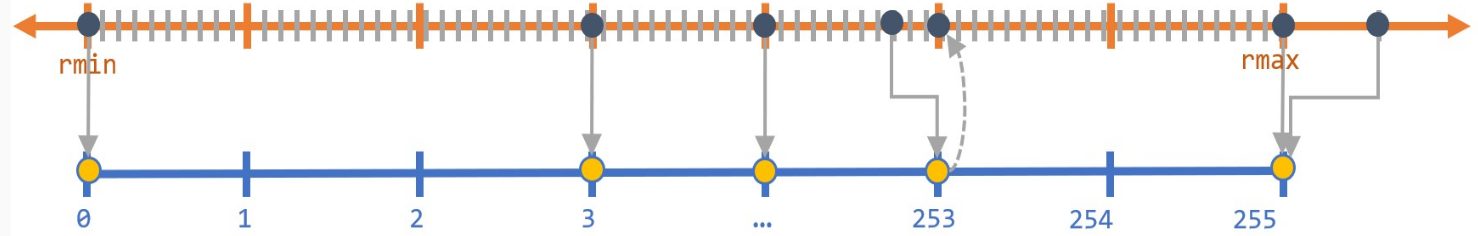
\includegraphics[scale=0.3]{inc/img/q8.jpg}
        \caption{Схема классической квантизации}
    \end{center}
\end{figure}

Будем называть уровнями квантизации вещественные значения, которые соответствуют всевозможным целочисленным квантизованным значениям $q$ параметра и определяются по формуле (1.1). Они обозначены оранжевыми штрихами на вещественной оси на рис.1.1.

Стоит обратить внимание на то, что в данной схеме $256$ уровней квантизации  распределены равномерно на отрезке минимального и максимального возможного значения параметра. Он определяется в процессе прогонки репрезентативной выборки реальных данных через исходную сеть. Процесс получения оптимальных  параметров квантизации для уже обученной модели при помощи прогонки через неё реальных данных, но без использования известных ответов, под которые обучалась сеть, будет называться в этой работе post-training квантизацией.

Перспективы, которые даёт квантизованное представление параметров:
\begin{itemize}
    \item Снижается объем вычислений за счет того, что операции сложения и умножения, которые используются в сетях, работают быстрее за счёт целочисленных вычислений и меньшего количества бит на одно число.
    \item Снижается размер, занимаемый сетью при вычислениях в оперативной памяти.
    \item Снижается размер, занимаемый сетью при хранении на жестком диске ЭВМ.
    \item Появляется возможность исполнения моделей на тех устройствах, в которых нет поддержки вещественной арифметики на уровне железа. Такими устройствами являются как микроконтроллеры компании ARM ниже версии Cortex Arm M4 в силу своей низкой стоимости и низкой производительности, так и высокоскоростные нейронные процессоры компаний Huawei и Qualcomm, которые берут на себя исполнение большинства нейронных сетей в современных телефонах и телевизорах. 
\end{itemize}

Однако очевидными являются и недостатки метода. Поскольку мощность поля вещественных чисел выше, чем ограниченного $2^K$ значениями множества целых чисел, где $K$ — количество бит для кодировки одного параметра,  легко догадаться, что данное преобразование будет вести к потерям точности работы обученной сети. Минимизация этой потери - основная задача инструмента, называемого квантизатором нейронных сетей, который выполняет это преобразование, подбирая наиболее оптимальные параметры квантизации $zp$ (zero point — точка, которой соответствует значение $0$ в вещественном поле) и $s$ (scale — коэффициент масштабирования). 

Равномерность распределения уровней квантизации является слабым местом классического алгоритма, поскольку распределение параметров в сети редко является равномерным, а имеет свою собственную природу, что будет показано далее. Этот факт является ограничителем для использования этого простого алгоритма для квантизации в представления с еще меньшим количеством бит, чем $8$, что демонстрируют результаты замеров, полученные в \cite{lq}, график которых показан на рис.1.2.

\begin{figure}[H]
    \begin{center}
        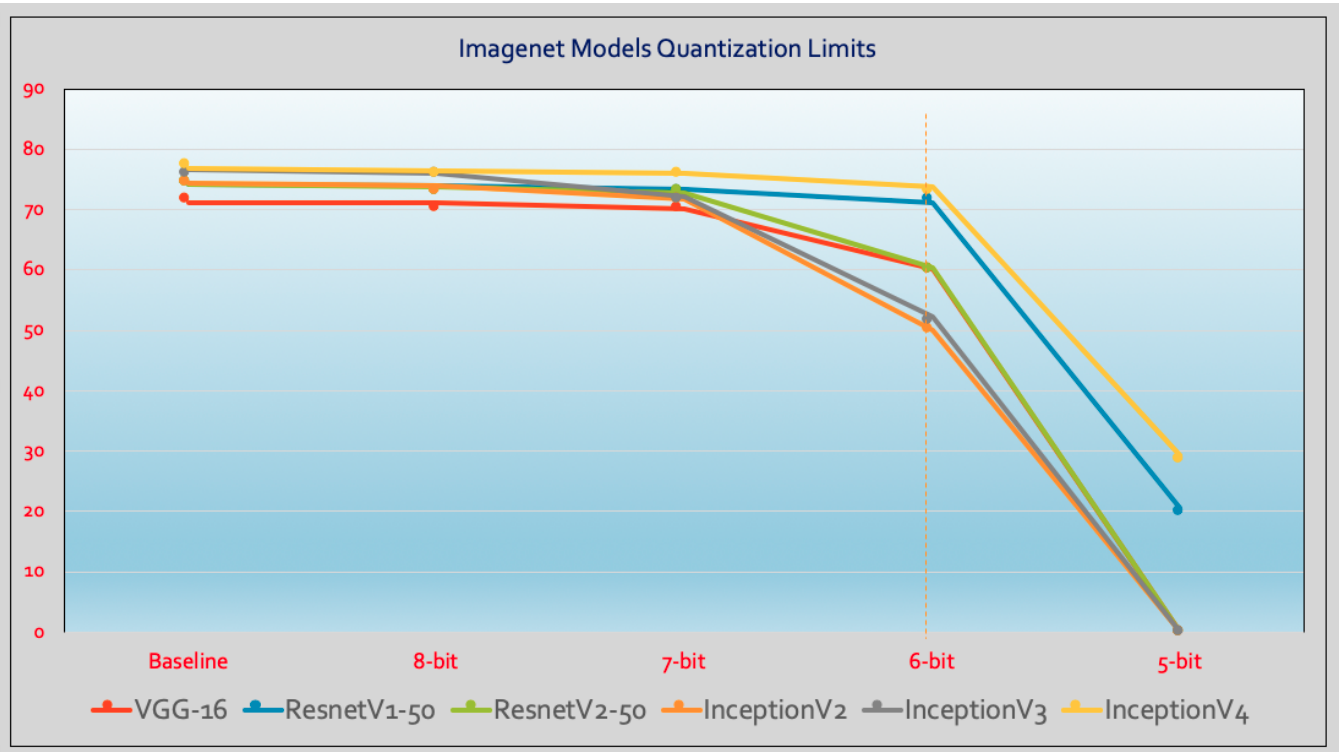
\includegraphics[scale=0.3]{tex/inc/img/q8stat.jpg}
        \caption{Точность моделей при уменьшении бит}
    \end{center}
\end{figure}

Этот же факт наталкивает на мысль о том, что для проведения более «экстремальной» квантизации с меньшим количеством бит на параметр, необходимо воспользоваться иными схемами интерпретации целого числа, которые будут лучше подстраивать уровни квантизации новой модели под распределение квантизуемых параметров. Именно о таком методе и будет идти речь в этой работе.

\section{Обучаемая квантизация}

Как уже было сказано выше, в данной работе вводится новый метод для квантизации сетей, который отличается от наиболее популярного и проверенного временем метода с равномерным распределением уровней квантизации. Перед предлагаемым алгоритмом квантизации, также как и перед любым другим, ставятся следующие задачи, которые он должен комплексно решать:

\begin{itemize}
    \item Определение оптимальных параметров квантизации как можно с меньшим количеством прогоняемых данных, затрачиваемых ресурсов и наибольшей сохраняемой  точностью модели.
    \item Возможность квантизации как можно в меньшие целочисленные размерности весов и активаций нейронной сети с целью уменьшения количества занимаемой памяти.
    \item Квантизация в такое представление, в котором эффективно производятся операции, тесно связанные с работой нейронных слоев, такие как перемножения матриц и свёртки.
\end{itemize}

По этой причине был выбран метод обучаемой низкобитовой post-training квантизации, который преобразует веса и активации глубокой модели в формат, позволяющий быстро и эффективно производить перемножения матриц при помощи побитовых операций. 

Суть этого метода заключается в том, что предлагается совершенно иной способ представления квантизованного числа в вещественом множестве. Обозначим кортеж $b = (b_0, b_1, ..., b_{K - 1}) \in \{ 0, 1 \}^K$ как бинарную запись квантизованного числа в Least Significant Bit first формате.  При классической квантизации одно $intK$ (где $K$ — количество бит для хранения одного значения) число $q$, вычисляемое по формуле (1.2), интерпретируется в действительном множестве как число $\overline{f}$ при помощи 2-ух параметров квантизации $s$ и $zp$ по формуле (1.1).

\begin{equation}
q = \sum \limits_{i = 0}^{K - 1} b_i 2^i
\end{equation}

В новом методе каждое квантизованное в $intK$ значение с бинарной записью $b$ интерпретируется согласно формуле (1.4), используя $a = (a_0, a_1, ..., a_{K-1})$ - вещественный базис-вектор коэффициентов для каждого из битов бинарного представления целого числа, имеющий длину $K$.

\begin{equation}
\overline{f} = \sum \limits_{i = 0}^{K - 1} b_i a_i,
\end{equation}

Иными словами, вещественное число, которое представлено квантизованным числом $q$ вычисляется как скалярное произведение базис-вектора из действительных чисел $a$ с бинарной записью этого квантизованного числа $b$. Базис-вектор $a$ будет являться настраиваемым параметром для отдельного слоя в процессе post-training квантизации. 

Следует оговориться, что из-за того,  что веса для каждого нейрона имеют разные распределения (что позволяет извлекать различные признаки из входных данных в рамках одного слоя), следует применять channel-wise квантизацию вместо layer-wise. Это означает наличие своего настраиваемого вещественного базис-вектора у каждого из нейронов слоя, вместо единого вектора для кодирования всех весов одного слоя.

С математической точки зрения это свойство не является обязательным, но в дальнейшем следует считать, что на значения базис-вектора $a$ накладывается строгое отношение частичного порядка: $a0 < a1 < ... < a_{K - 1}$. Это свойство дает возможность быстро определять отсортированные уровни квантизации <<на лету>>, что является важным свойством с при реализации.

Стоит отметить, что предлагаемый метод дает возможность интерпретировать биты числа не только в привычном множестве возможных значений $\{ 0, 1 \}$, но и в $\{ -1, 1 \}$, что позволяет уровням подстраиваться под отрицательные значения. Именно вариант $\{ -1, 1 \}$ будет использоваться в дальнейшем в данной работе. 

Описанная схема интерпретации числа $q$ на множестве действительных чисел имеет следующее преимущество: уровни квантизации накладываются не равномерно, а могут подстраиваться под конкретное распределение квантизуемого параметра. Например, если веса нейрона имеют стандартное распределение, то уровни квантизации должны иметь большую концентрацию  ближе к математическому ожиданию, что позволит точнее представлять величины, которые встречаются в сети наиболее часто. Пример вычисления и распределения уровней квантизации на числовой оси для $3$-х битной квантизации показан на рис.1.3.

\begin{figure}[H]
    \begin{center}
        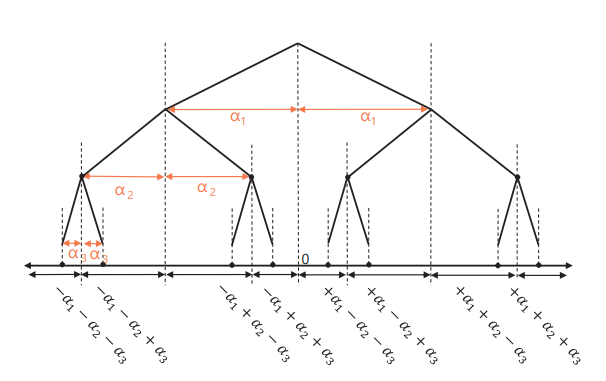
\includegraphics[scale=0.55]{tex/inc/img/lvls.jpg}
        \caption{Распределение уровней квантизации}
    \end{center}
\end{figure}

Если посмотреть на гистограмму весов в каналах слоёв нейронной сети для задач компьютерного зрения ResNet-20, полученное в работе \cite{lq}, становится понятно, что такой способ представления квантизованных значений точнее описывает генеральное распределение параметров.

\begin{figure}[H]
    \begin{center}
        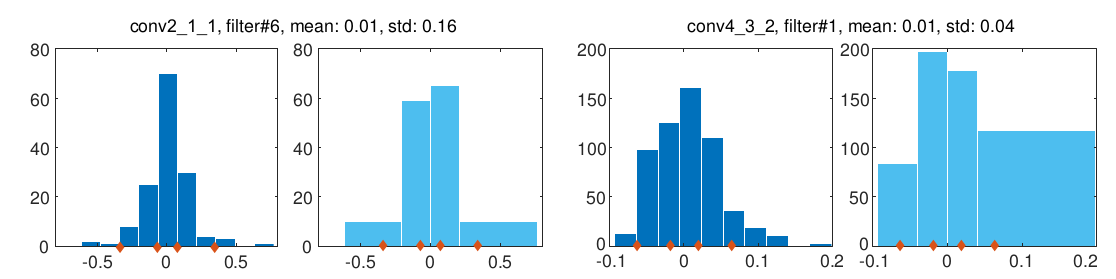
\includegraphics[scale=0.36]{tex/inc/img/distrib.jpg}
        \caption{Распределение весов в ResNet-20}
    \end{center}
\end{figure}


На рис. 1.4. точками оранжевого цвета показано, как можно оптимально разместить уровни при описанном способе кодировки вещественных величин для $2$-х битной квантизации весовых параметров. Следует обратить внимание на то, что веса в разных каналах слоя имеют разные распределения, что является обоснованием для выбора channel-wise преобразования вместо layer-wise, о чем было упомянуто выше.

Стоит не забыть упомянуть, что количество уровней квантизации для $intK$ равно $2^K$, а сами уровни получаются в результате применения формулы (1.4) ко всевозможным комбинациям бинарных записей из $K$ бит.

\begin{figure}[H]
    \begin{center}
        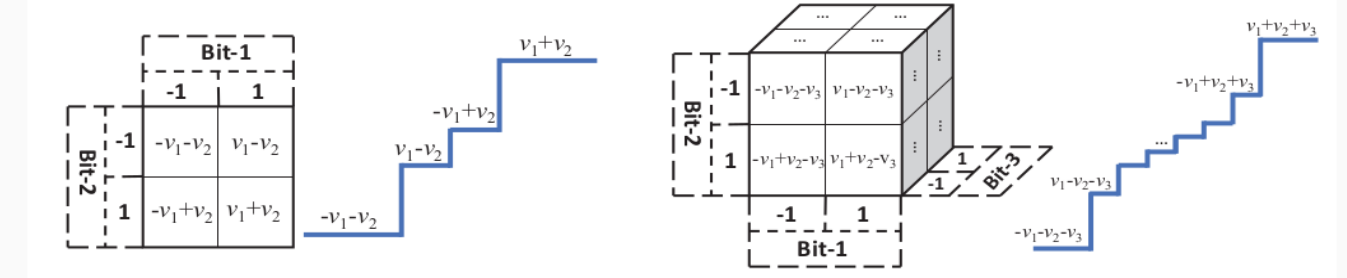
\includegraphics[scale=0.35]{tex/inc/img/lvls2.jpg}
        \caption{Уровни квантизации}
    \end{center}
\end{figure}

Возникает вопрос не только, как интерпретировать имеющееся квантизованное число в вещественном представлении, но и каким целочисленным значением оптимальнее всего представить число с действительной оси. Эта часть описываемого алгоритма идентична тому, как аналогичное преобразование производится для классической $8$-битной квантизации, однако стоит рассмотреть этот этап поподробнее. Сначала на основе базис-вектора $a$ определяются уровни квантизации $q_l = (a, e_l), \; \forall e_l \in \{ -1, 1 \}^K$, такие что $q_0 < q_1 < ... < q_{2^K}$, и на основе них рассчитываются пороги  $t_l = \displaystyle\frac{q_l + q_{l-1}}{2}$, с помощью которых определяется к какому уровню следует отнести конкретное число, как показано на рис.1.6. 

\begin{figure}[H]
    \begin{center}
        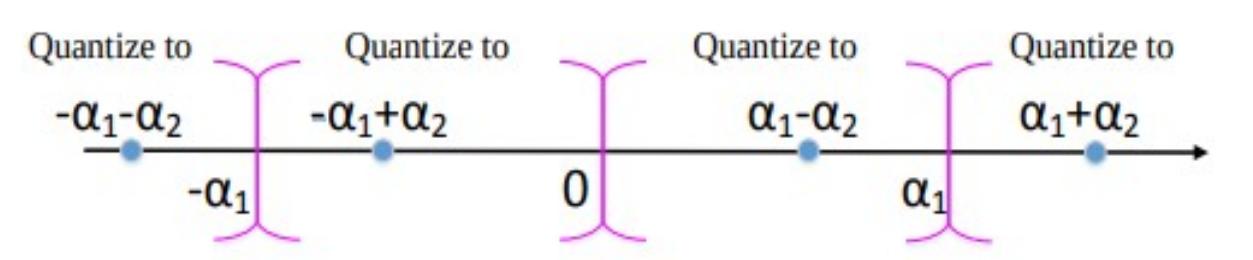
\includegraphics[scale=0.3]{tex/inc/img/define.jpg}
        \caption{Определение оптимальной кодировки}
    \end{center}
\end{figure}

После определения уровня квантизации  при помощи порогов, следует взять соответствующую бинарную кодировку, которая будет являться оптимальным квантизованным значением для исходного вещественного числа.

Для того, чтобы уровни могли распределяться не только вокруг $0$, но и любого другого числа (ведь распределение значений параметра может быть смёщенным), следует добавить свободный коэффициент смещения к обучаемому базис-вектору, что даст дополнительную степень свободы описываемому алгоритму. Однако исследование и решение этой проблемы не затрагивается в данной работе.

У метода есть явный недостаток — большое количество настраиваемых аргументов, равное сумме длин всех базис-векторов. Издержки на хранение таких векторов в памяти достаточно малы по сравнению с количеством весовых значений, поэтому их можно не брать в учет при анализе метода. Но обучение  при таком числе параметров квантизации становится трудной задачей, требующей применения различных эвристик, которые позволяют находить оптимумы в вещественных пространствах больших размерностей.

Как было заявлено и будет показано далее в описании работы нового слоя, такой вариант преобразования параметров даёт возможность быстрого матричного перемножения квантизованных весовых и входных значений. Среди огромного разнообразия существующих операций, встречающихся в глубоких моделях на текущий момент, наиболее ярко выделяются полносвязные слои, рекуррентные, свёрточные и субдискретизационные. Именно на работе этих операций построена любая современная нейронная сеть, поэтому на них следует делать упор при оптимизации работы моделей, в том числе и в квантизации. 

Упомянутые субдискретизационные слои являются довольно быстрой операцией, работающей за $O(n)$ от размера входных данных, и издержки на проведение квантизации с учётом потери точности слишком велики по сравнению с выгодой, которую может дать предлагаемое преобразование. Рекуррентные сети, такие как GRU, LSTM, RNN, описанные в \cite{gru}, \cite{lstm}, \cite{rnn} соответственно, содержат внутри своей реализации полносвязные нейронные слои. Что касается свёрточных слоев, про которые подробно рассказывается в \cite{conv}, то операция свёртки в них может быть сведена к перемножению двух матриц (GEMM) при помощи im2col преобразования. Эта техника, описанная в \cite{im2col}, зачастую применяется, поскольку позволяет добиться значительного увеличения скорости работы таких слоёв за счет того, что алгоритм перемножения матриц оптимальнее работает с кешом процессора, благодаря последовательному доступу к памяти.  Именно поэтому в данной работе было решено акцентировать внимание на проведение квантизации с классическим полносвязным слоем, поскольку все остальные существующие операции либо содержат такой слой внутри себя, либо могут быть приведены к такому формату, либо издержки и потери превалируют над возможным выигрышем от преобразования, поскольку не содержат в себе ресурсоёмких матричных произведений. Все слои сети, отличные от полносвязных, будут оставаться без изменений в данной работе.

Описанный в \cite{rnn} классический полносвязный нейронный слой — это набор из нейронов, реализующих в себе алгоритм линейной регрессии вместе с функцией активации, которая призвана добавить нелинейности к выходу нейрона и придать системе большую устойчивость за счет асимптотических ограничений, накладываемых на выход нейрона. Количество таких нейронов задается тем, кто обучает подобный слой. Как нетрудно догадаться, оно равно размерности выходного вектора (output), который выдает слой на основе входного вектора данных (input). Схематично нейрон сети может быть представлен схемой на рис. 1.7.

\begin{figure}[H]
    \begin{center}
        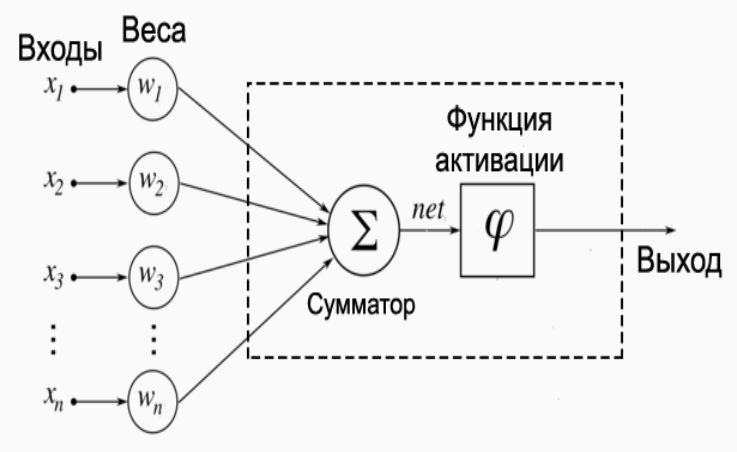
\includegraphics[scale=0.3]{tex/inc/img/neron.jpg}
        \caption{Нейрон}
    \end{center}
\end{figure}

В то же самое время показанная схема эквивалентна вычислению функции активации $\sigma$ от суммы между скалярным произведением входов слоя $x$ с вектором весов нейрона $w$ и смещением для $i$ - го нейрона по формуле (1.5).

\begin{equation}
y_i = \sigma((x_i, w_i) + b_i), \; \forall i: 0 < i < m
\end{equation}

Выход такого нейрона — скаляр $y_i$, называемый выходом нейрона.

Формулу (1.5) можно расширить в более общий случай, когда на вход поступает несколько входных векторов в виде матрицы $X$ и используется целый полносвязный нейронный слой из $m$ описанных выше нейронов, веса которых также могут быть объединены в единую матрицу $W$, столбцы в которой — весовые вектора для отдельного нейрона. Тогда выходную матрицу $y = (y_0, y_1, ..., y_{m - 1})$ можно рассчитать при помощи результата произведения матрицы весов на матрицу входов, к каждой строке которого добавляется вектор смещений $b = (b_0, b_1, ..., b_{m-1})$, состоящий из свободных коэффициентов каждого нейрона слоя, и поэлементно применяется функция активаций $\sigma$, что отображено в (1.6).

\begin{equation}
y = \sigma (XW + b)
\end{equation}

\begin{figure}[H]
    \begin{center}
        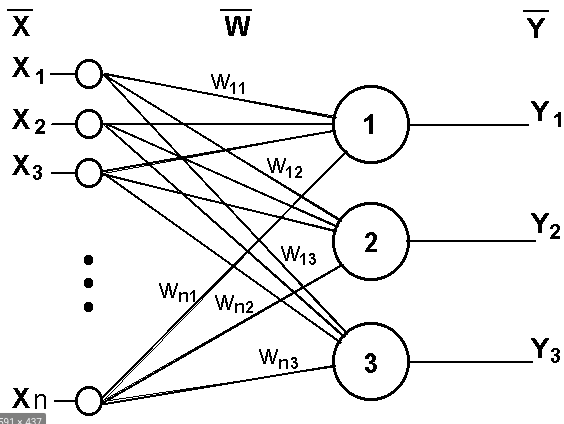
\includegraphics[scale=0.3]{tex/inc/img/layer.jpg}
        \caption{Полносвязный слой}
    \end{center}
\end{figure}

Основываясь на специфике работы слоя, проиллюстрированного рис. 1.8., можно выделить следующие параметры нейронного слоя, которые необходимо хранить и использовать при расчетах:

\begin{itemize}
    \item Веса модели в виде матрицы $W \in R^{n \times m}$, где $n$ - размер входных векторов, а $m$ - количество нейронов.
    \item Вектор из смещений всех нейронов $b \in R^{m}$.
    \item Тип функции активации $\sigma$, которая применяется к каждому значению выходного вектора.
\end{itemize}

Поскольку смещения занимают мало места в памяти и сложение происходит за $O(n)$, квантизовать их не имеет смысла. Зато весовые параметры составляют наибольшую часть занимаемого сетью объема, а время на перемножение весов на матрицу входов $X$ является самой ресурсоемкой операцией, оптимизировать которую можно в квантизованных вычислениях, используя побитовую арифметику. 

Как было показано выше, поскольку у каждого из нейронов свое распределение весов, то квантизовать следует каждый из его весовых векторов отдельно. При этом в данном методе затрачивается $K_w$ битов на квантизацию каждого веса нейрона. Тогда каждый весовой вектор нейрона может быть представлен бинарной матрицей $B^w \in \{ -1, 1\}^{K_w \times n}$, где каждому весу исходного вектора соответствует бинарный столбец, означающий его квантизованное значение.  Каждый входной вектор (строка матрицы $X$) также может быть представлен в бинарном виде $B^x \in \{ -1, 1 \}^{K_x \times n}$  при помощи отдельных параметров квантизации для входов слоя. Следует сразу отметить, что количество бит $K_w$ на кодирование весов может не совпадать с количеством $K_x$, используемым для кодирования входных значений.

В таком случае, результат скалярного произведения входного и весового вектора в квантизованных вычислениях будет расчитываться по формуле (1.7).

\begin{equation}
\sum\limits_{k = 1}^{n} x_k w_k \approx \sum\limits_{k = 1}^{n}\sum\limits_{i = 1}^{K^x} (b^x_{ik} a^x_i) \sum\limits_{j = 1}^{K^w} (b^w_{jk} a^w_j) = \sum\limits_{i = 1}^{K^x}\sum\limits_{j = 1}^{K^w} a^x_i a^w_j (\sum\limits_{k = 1}^{n} b^x_{ik} b^w_{jk}),
\end{equation}

где $b^x_{ik}$ и $b^w_{ik}$ - бит, находящийся на $i$-ой строке в $k$-ом столбце бинарной матрицы $B^x$ и $B^w$ соответственно. 

Обозначим $i$-ую строку бинарной матрицы $B^x$ и $B^w$ как $b^x_{i}$ и $b^w_{i}$ соответственно, а под оператором $\odot$ будем понимать скалярное произведение двух бинарных векторов. В таком случае формулу (1.7) можно переписать в виде (1.8).

\begin{equation}
\sum\limits_{k = 1}^{n} x_k w_k \approx \sum\limits_{i = 1}^{K^x}\sum\limits_{j = 1}^{K^w} a^x_i a^w_j (b^x_{i} \odot b^w_{j}),
\end{equation}

Для обоснования выигрыша в скорости, который дает предложенная формула для расчета, следует подробнее рассмотреть бинарное скалярное произведение.

 Скалярное произведение — сумма произведений соответствующих элементов двух векторов. В это же время бинарное множество $\{ -1, 1 \}$ замкнуто относительно операции умножения, поэтому произведение двух бинарных значений остается бинарным значением, а значит может быть представлено одним битом. Возможны следующие варианты произведения $2$-ух битов:

\begin{enumerate}[label=\arabic*.]
    \item $-1(0) \cdot -1(0) = 1(1)$
    \item $-1(0) \cdot 1(1) = -1(0)$
    \item $1(1) \cdot -1(0) = -1(0)$
    \item $1(1) \cdot 1(1) = 1(1)$
\end{enumerate}

Такой схеме соответствует бинарная операция $xnor = \lnot xor$, логическая схема которой представлена на рис. 1.9.

\begin{figure}[H]
    \begin{center}
        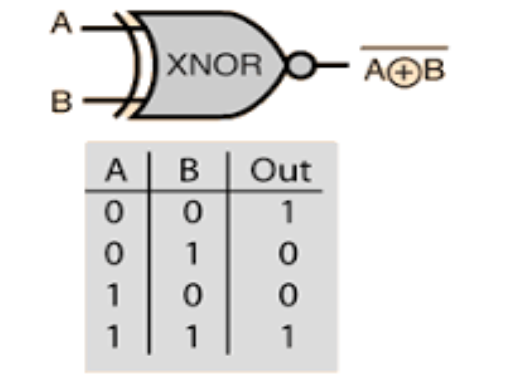
\includegraphics[scale=0.3]{tex/inc/img/xnor.jpg}
        \caption{Xnor}
    \end{center}
\end{figure}

Тогда в результате применения побитового xnor к двум бинарным векторам получается вектор, подсчет скалярного произведения из которого сводится к разности количества единиц в нем и количества нулей ($-1$ в принятом соглашении). Для подсчета количества единиц в бинарной записи числа в наборах инструкций современных архитектур ЭВМ существуют соответствующаие инструкции, такие как POPCNT в SSE4.2 Intel \cite{intel} и VCNT в Arm NEON \cite{neon}. Решив простую систему уравнений (1.9), можно получить формулу (1.10).

\begin{equation}
 \begin{cases}
 \odot = pos - neg
 \\
 size = pos + neg,
 \end{cases}
\end{equation}

\begin{equation}
 \odot = 2 pos - size
\end{equation}

где $pos$ — количество $1$ в строке, $neg$ — количество $-1$ в строке, $size$ -  размер строки в битах. 

Следовательно, результат бинарного скалярного произведения может быть посчитан с использованием (1.10) при помощи описанных выше побитовых операций. Формула (1.11) — бинарное скалярное произведение 2-ух строк матриц закодированных весов.

\begin{equation}
b^x_{i} \odot b^w_{j} = 2 popcnt(\lnot(b^x_i \oplus b^w_j)) - size
\end{equation}

Каждая из операций в (1.11) поддержана в современных архитектурах на уровне железа, что делает эту часть скалярного произведения крайне эффективной с вычислительной точки зрения.

Эффективность предложенного метода для расчета выходов нейронов ожидается не только при выполнении нейронных сетей на классических архитекутах процессоров, но и при реализации полносвязного слоя с использованием мемристорных кроссбаров. Реализация бинарного скаляного произведения на схеме с использованием мемристорных элементов приводится в \cite{memristor}. Поскольку мемристор имеет ограниченное количество уровней проводимости, матричные произведения на кросcбарах необходимо также выполнять в дискретизованном формате, что предполагает использование низкобитовой квантизации. Исследование потери точности при уменьшении количества уровней дискретизации приведено в работе \cite{discret}, где обосновывается возможность использования кроссбаров для задач глубокого обучения.

Поскольку ЭВМ способны оперировать типами данных ограниченного размера, то при условии хранения строк бинарных матриц в виде массива 32-битных целых чисел uint32, псевдокод быстрого бинарного скалярного произведения в с++20 представлен в листинге 1.1.


\begin{lstlisting}[language=C++, caption={Пример модели с LQFullyConnected}]
int32_t bin_dot(uint32_t* b_a, uint32_t* b_w, uint32_t neurons){
  uint32_t size = (neurons + 31) >> 5; // ceil divide to 32
  int32_t pos = neurons - (size << 5);
  for(uint32_t i = 0; i < size; ++i){
    pos += std::popcount(~(b_a[i] ^ b_w[i])); // popcnt(xnor)
  }
  return (pos << 1) - neurons;
}
\end{lstlisting}

Опираясь на полученную арифметику оптимального перемножения и на соображения кэш-дружелюбности при вычислениях, принято решение хранить в квантизованных слоях веса в бинаризованном формате в виде $3$-х мерного целочисленного тензора с размерами: $(o, k, ceil(n / 32))$, где $o$ — размер выходного вектора, $k$ — количество бит для кодирования каждого веса, $n$ — размер входного вектора. Деление с округлением вверх в определении размера $3$-го измерения предусматривает случаи, когда размер входного вектора $n$ не делится на $32$ целочисленно. Базис-векторы для весов следует хранить в виде вещественного тензора размера $(o, k)$ для более эффективного доступа к ним во время вычисления аппроксимированного скалярного произведения по выведенной выше формуле, а базис-вектор для кодирования входных значений может быть представлен в виде одномерного вещественного тензора, длина которого совпадает с количеством бит на кодирование одного входного значения.

\begin{figure}[H]
    \begin{center}
        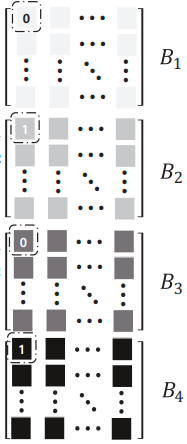
\includegraphics[scale=0.35]{tex/inc/img/bindata.jpg}
        \caption{Бинарные веса для 4 нейронов}
    \end{center}
\end{figure}

Как нетрудно догадаться, на вход слоя поступает матрица в неквантизованном виде, потому что входной вектор слоя напрямую зависит от тех вещественных данных, что приходят на вход всей нейронной сети, что делает невозможным квантизацию входов до начала исполнения модели и вынуждает проводить преобразование в бинарное представление во время работы нейронной сети каждый раз перед вычислением выходов нейронов слоя. Это является одним из существенных недостатков алгоритма, но даже несмотря на это этот казус, алгоритм остается крайне эффективным, поскольку время, которое тратится на квантизацию можно асимптотически оценить как O(n k), поскольку для каждого входного значения определяется набор бит, которые оптимально его кодирует с помощью бинарного поиска по массиву порогов квантизации, что делается за $O(log(2^K)) = O(K)$, после чего квантизованное значение записывается побитово в  буффер, на что также требуется $O(K)$ по времени.

Ранее уже было упомянуто, что задача квантизации — как можно сильнее снизить потери от перевода значений из области действительных чисел в целые числа. Для достижения этой цели базис-векторы обучаются таким образом, чтобы минимизировать ошибку между реальным вещественным значением и соответствующим его квантизованному значению действительным числом. Пусть $Q(x)$ - функция-квантизатор, которая возвращает для действительного числа $x$ его оптимальный уровень квантизации. Тогда, если описать решаемую описываемым инструментом проблему более формально, то нам необходимо найти оптимальный квантизатор, который минимизирует математическое ожидание квадратической ошибки для параметра, распределённого с плотностью $p(x)$.

\begin{equation}
Q^{*} = \argmin \limits_Q \int \limits_{- \infty}^{\infty} p(x) (Q(x) - x)^2 dx
\end{equation}

Решение этой проблемы аналитически почти всегда невозможно из-за того, что закон распределения  генеральной совокупности параметров при квантизации не известен, а поиск решения этой проблемы через линейный поиск по параметрам квантизации может занять слишком много времени. Поэтому в этом методе предлагается использовать эвристический алгоритм QEM(Quantization Error Minimization). Этот алгоритм, описание которого приводится в \cite{lq}, работает с исходным вещественным вектором входных данных $x$ и итеративно пытается улучшить значение базис-вектора $a$, основываясь на наилучшем значении этого вектора для промежуточной кодировки  $B$.

Алгоритм QEM:
\begin{enumerate}[label=\arabic*.]
    \item Инициализировать $a$ случайными значениями.
    \item Повторять от $0$ до $T$:
    \begin{enumerate}[label=\arabic*.]
    \item Найти оптимальную промежуточную кодировку $B^*$ для $x$ на основе $a$.
    \item Найти оптимальный $a^* = \argmin \limits_a \| B^* a - x \|^2$ и обновить $a$ полученным значением $a^*$.
    \end{enumerate}
\end{enumerate}

Поиск оптимальной матрицы в пункте 2.1 определяется процессом квантизации с использованием порогов, который был описан выше. Что касается пункта 2.2, то при справедливости условий Маркова-Гаусса (что на практике, к сожалению, не часто выполняется) оптимальный базис-вектор может быть найден при помощи метода наименьших квадратов по формуле (1.13), что и предлагается в \cite{lq}. 

\begin{equation}
a^* = (B B^T)^{-1} Bx
\end{equation}

Так как операция обращения матрицы является вычислительно емкой и трудно гарантировать, что определитель матрицы ковариаций $B B^T$ не будет равен или близок к $0$ в процессе обучения, поэтому в данной работе предлагается использовать итеративный градиентный спуск с $L_2$ регуляризацией, на каждой итерации которого значения будут обновляться следующим образом по формуле (1.14).

\begin{equation}
a = a - \frac{lr}{n} \sum \limits_{i = 1}^{n} [((b_i, a) - x_i)b_i + \lambda a],
\end{equation}

где $b_i$ - $i$-ый столбец матрицы $B$, $а$ - темп обучения, который задается в качестве гиперпараметра и регулирует скорость сходимости алгоритма к оптимуму. Регуляризация с параметром $\lambda$ используется чтобы штрафовать большие значения параметров, потому что веса и входы слоёв, как правило, имеют небольшие значения.

Применение данного алгоритма для обучения базис-вектора параметров предлагается в данной работе как основа инструмента для post-training квантизации. Этот метод обучения работает не только в предлагаемом методе работы с весами и активациями слоя. Он может определять оптимальные значения параметров для других методов, например BiQGEMM из \cite{bqgemm},  в котором предлагается иной способ  расчета результата генерального матричного произведения без перевода входных значений в целочисленный вид, но совпадает формат хранения и интерпретация весов слоя. 
\chapter{Практическая часть}
\label{cha:ch_2}


При выборе базового фреймворка для реализации функциональности, описанной в теоретической части следовало опираться на следующие факторы:

\begin{itemize}
    \item Открытый и понятный исходный код с лицензией, позволяющей добавление собственного программного кода.
    \item Наличие собственного формата in-memory представления нейронной сети.
    \item Наличие формата и инструментов для сериализации/десериализации глубоких моделей.
    \item Наличие легковесного интерпретатора для нейронных моделей, который можно расширить добавлением собственных вычислительных ядер для интерпретации новых нейронных слоёв. 
    \item Наличие инструментов, которые позволяют переводить глубокие модели во внутренний формат из других популярных форматов, в которых могла быть обучена исходная нейронная сеть.
\end{itemize}

Среди проектов, соответствующих выделенным критериям, ярко выделяются такие, как Tensorflow от компании Google и ONE от компании Samsung. Выбор был сделан в пользу последнего, поскольку он активно развивается под лицензией Apache 2.0, а его интерпретатор показывает лучшие результаты в проведенных бенчмарках на ЭВМ с жесткими ограничениями в ресурсах за счет лучшей работы с памятью.

Разработка велась в локальном форке исходного проекта на GitHub в отдельной ветке (URL: https://github.com/Bronnikoff/ONE/tree/lq\_nets), поскольку это удобный способ управлять добавляемым кодом при определенной независимости от параллельных изменений, вносимых в базовый проект со стороны его разработчиков.

\section{Поддержка слоя в графовых представлениях}

Квантизованный слой имеет отличное от оригинального слоя поведение при вычислениях, количество параметров и формат хранения данных. Это означает, что для поддержки его работы и для удобства обработки графа при написании квантизатора, необходимо поддержать новую операцию LQFullyConnected во всех имеющихся в ONE графовых представлениях, которые используются для работы с моделью от этапа её считывания из файла до этапа расчета результатов ее работы. Префикс LQ (Learnable Quantization), содержащийся в названии операции, был добавлен к названию чтобы указать на то, что она является результатом перевода полносвязанного (FullyConnected) слоя в низкобитовый формат при помощи обучаемых параметров квантизации.


Такими графовыми представлениями, через которые проходит модель до непосредственного запуска, являются:
\begin{itemize}
    \item Представление circle для сериализации и десериализации графовых моделей с жёсткого диска.
    \item In-memory представление luci, которое работает со слоями как с вершинами, соединенными друг с другом посредством указателей.
    \item Вычислительный граф, который оперирует тензорами, связанными друг с другом вычислительными ядрами операций.
\end{itemize}

Реализацию было решено начать с описания схемы хранения квантизованного слоя в долгосрочной памяти  вместе со схемой его сериализации и десериализации (способа записи структуры данных на жесткий диск и извлечения её из него). Благодаря тому, что принятый в Samsung формат хранения моделей circle основан на известной технологии flatbuffers, этот этап потребовал лишь описания в файле circle-schema.fbs параметров, которые уникальны и присущи только добавляемому слою. 

\begin{lstlisting}[language=C++, caption={Структура слоя в схеме}]
table LQFullyConnectedOptions {
	hidden_size: int;
	fused_activation_function:ActivationFunctionType;
}
\end{lstlisting}

Этими параметрами являются тип функции активации, которая применяется к выходу сумматора каждого нейрона и число hidden\_size, равное размеру входного вектора, поскольку его необходимо знать в случаях, когда размер входных данных не делится на цело на 32, для корректного расчета бинарных скалярных произведений при работе операции.

Помимо описания уникальных параметров LQFullyConnected, требуется декларировать наличие этого нового оператора и присвоить ему уникальный номер в схеме формата circle, который был выбран случайным образом.

Остальная работа по сохранению и извлечению модели производится самим flatbuffers. При помощи компилятора flatc, предоставляемого компанией Google, на основе схемы, которая была расширена параметрами нового слоя, генерируется хедер-файл для языка С++. Этот файл schema\_generated.h реализовывает алгоритм перевода набора байт из дискового пространства в описанную в С++ структуру хранения этой операции в памяти при работе программы, извлекая в том числе и информацию о связях с соседними операциями в графе модели. Стоит отметить, что flatc поддерживает несколько языков программирования, таких как Java или JS, а не только C++, что позволяет работать с circle не только в C++. Применение этого свойства будет показано далее.

После того, как новая операция была добавлена в circle, следует перейти к поддержке LQFullyConnected в основном промежуточном представлении (Intermideate Representation) под названием luci. В отличие от 2-ух других представлений, оно не создано для решения какой-то конкретной задачи, такой как высокопроизводительный запуск сети или реализация алгоритмов работы с сырыми данными из файла. Поэтому в нём модели представлены в виде классических графов, вершинами которых являются операции, а связи между соседними слоями прописаны явно, через указатели языка C++. Универсальный вид графа делает его удобным для применения различных оптимизаций с подграфами модели. Также из него удобно перевести модель в любой другой формат, который заточен под решение конкретной задачи.

Следует выделить 4 основных части в формате luci:
\begin{enumerate}[label=\arabic*.]
    \item Описание представления каждой операции в формате. (luci/lang)
    \item Функциональность для импорта модели из circle. (luci/import)
    \item Функциональность для экспорта модели из circle. (luci/export)
    \item Алгоритмы оптимизации, применяемые к графу. (luci/pass)
\end{enumerate}

На уровне описания структуры представления LQFullyConnected в luci, отраженной на листинге 2.2, явно объявляется, что новая операция должна иметь 5 входных вершин: входная вершина, из которой поступают входные данные, базис-вектор для квантизации входных данных, набор базис-векторов для квантизации весов слоя, бинаризованные веса и вектор смещений.

\begin{lstlisting}[language=C++, caption={Структура слоя в luci}]
class CircleLQFullyConnected final : public FixedArityNode<5, 
    CircleNodeImpl<CircleOpcode::LQ_FULLY_CONNECTED>>,
    public CircleNodeMixin<CircleNodeTrait::FusedActFunc>,
    public CircleNodeMixin<CircleNodeTrait::Bias>
{
public:
  loco::Node *input(void) const { return at(0)->node(); }
  void input(loco::Node *node) { at(0)->node(node); }

  loco::Node *input_scales(void) const { return at(1)->node(); }
  void input_scales(loco::Node *node) { at(1)->node(node); }

  loco::Node *weights_scales(void) const { return at(2)->node(); }
  void weights_scales(loco::Node *node) { at(2)->node(node); }

  loco::Node *weights_binary(void) const { return at(3)->node(); }
  void weights_binary(loco::Node *node) { at(3)->node(node); }

  loco::Node *bias(void) const override { return at(4)->node(); }
  void bias(loco::Node *node) override { at(4)->node(node); }

public:
  int32_t weights_hidden_size(void) const { 
    return _weights_hidden_size; 
  }
  void weights_hidden_size(int32_t weights_hidden_size)
  {
    _weights_hidden_size = weights_hidden_size;
  }

private:
  int32_t _weights_hidden_size = 0;
};
\end{lstlisting}

Стоит отметить, что luci явно не требует, чтобы все из входных вершин существовали. Например, bias() может принимать значение nullprt. 

Основная функциональность для перевода моделей из luci в circle и обратно уже была реализована внутри проекта профессионалами из Samsung, что потребовало тривиальных изменений в исходном коде для поддержки импорта и экспорта.

Оптимизации для подграфов, содержащих LQFullyConnected в данной работе не рассматриваются, поэтому единственные алгоритмы, которые потребовалось реализовать в luci/pass — это определение типа данных (TypeInferencePass) и алгоритм определения размерности выходов слоя на основе размеров входных вершин (ShapeInferencePass).

Опциональной частью этой работы стала модификация существующего в проекте кода, отвечающего за отображение свойств операции в текстовом формате. Помимо этого, было полезно иметь наглядную визуализацию сетей, в графе которых присутствует добавляемая в этой работе операция. Для этого был модифицирован исходный код другого популярного проекта для визуализации множества различных нейросетевых форматов netron, который работает на языке JS. Как было отмечено ранее, flatc умеет переводить схему не только в C++, но и в JS. Сгенерированная с помощью flatc в JS схема работы с форматом circle была добавлена в этот инструмент, а остальная функциональность для работы с этой схемой уже присутствовала в «исходниках» визуализатора, поскольку он уже поддерживает формат tflite, который также основывается на flatbuffers.

При помощи описания простой нейронной сети с одним входом, одной LQFullyConnected операцией и одним выходом, при использовании имеющегося в проекте ONE инструмента circlechef для перевода описаний моделей в реальные физические модели, был получена первая сеть, визуализация которой netron-ом дала результат на рис. 2.1.

\begin{figure}[H]
    \begin{center}
        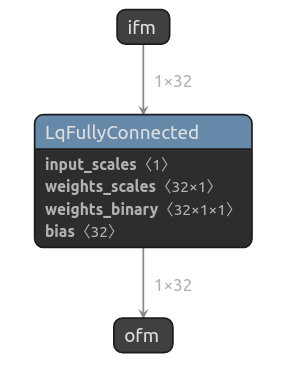
\includegraphics[scale=0.4]{tex/inc/img/lq.png}
        \caption{Пример модели с LQFullyConnected}
    \end{center}
\end{figure}

Возможность анализа моделей посредством визуализатора не входит в данную работу как необходимая ее часть, однако позволяет увеличить удобство работы пользователя с сетями в формате circle и ускорить дальнейший процесс разработки и отладки кода.

Последним из выделенных графовых представлений является форма вычислительного графа, которая спроектирована таким образом, чтобы минимизировать издержки при работе с слоями и достичь максимальной производительности. Вершинами в этом представлении являются тензоры, связанные между собой вычислительными ядрами. Для того, чтобы поддержать операцию на этом уровне, необходимо определить класс для операции, инкапсулирующий в себе разные вычислительные ядра в зависимости от типа поступающих данных и описывающий логику взаимодействия тензоров между собой.

Такой класс помимо ядер и указателей на входные и выходные тензоры содержит метод configure(), который необходимо переопределить для:

\begin{itemize}
    \item Проверки, что со входными тензорами можно провести запуск ядра. Именно в этом месте накладываются ограничения на параметры квантизованного слоя, описанные и обоснованные в теоретической части этой работы.
    \item Определения размерности данных, с которыми необходимо оперировать вычислительному ядру, и аллоцирования выходного тензора.
    \item Создания и инициализация вспомогательных вычислительных структур. Здесь создается объект класса LQBinarizer, инкапсулирующий в себе квантизацию входных данных вместе буфером для его квантизованных значений.
\end{itemize}

\section{Вычислительное ядро интерпретатора}

Вычислительное ядро интерпретатора вычисляет выходы операции LQFullyConnnected на основе входных данных, находящихся в тензоре input. Поскольку поступающие входные данные являются вещественными, а не квантизованными, перед расчетом выхода отдельного нейрона для одного входного вектора по формуле (1.8) необходимо произвести квантизацию входного вектора, с целью получения закодированного int32 буфера, который будет использоваться при расчетах. В связи с этим следует рассмотреть 2 основные части, которые требуется реализовать для поддержки корректной работы интерпретатора с моделями, содержащими LQFullyConnected:

\begin{itemize}
    \item Класс LQBinarizer, позволяющий проводить кодирование входных вещественных векторов и предоставляющий доступ к бинарным данным.
    \item Функция evalFloat, производящая расчет выходов по формуле (1.8), используя LQBinarizer внутри себя.
\end{itemize}

\subsection{Кодировщик LQBinarizer}

Для квантизации входных значений <<на лету>> появилась необходимость ввести вспомогательный класс LQBinarizer, объявление которого показано на листинге 2.3.

\begin{lstlisting}[language=C++, caption={Класс кодировщика}]
class LQBinarizer
{
  using Level = std::pair<float, int32_t>;

public:
  LQBinarizer(int32_t data_vec_size, const Tensor *data_scales);

  const int32_t *data() { return data_binary.get(); }

  void quantize_and_pack(const float *data_vector);

private:
  int32_t bin_search_encoding(float value);

private:
  int32_t data_float_size;
  int32_t data_bin_size;
  int32_t encode_bits;
  std::unique_ptr<int32_t[]> data_binary;

  int32_t levels_count;
  std::unique_ptr<Level[]> quantization_levels;
  std::unique_ptr<float[]> quantization_thresholds;
};
\end{lstlisting}

В конструкторе класса определяются пороги и уровни квантизации в отсортироанном порядке. Они необходимы для определения оптимальной кодировки для каждого из вещественных чисел. Помимо этого, при создании объекта класса происходит аллокация буфера бинарных данных и определяется чило $data\_bin\_size = ceil(data\_float\_size / 32)$, которое равно длине одной строки выделенного буфера. Было решено сделать выделение памяти за один раз в конструкторе, связав её освобождение с концом жизни объекта кодировщика через умные указатели, чтобы снизить издержки на ее перевыделение при расчете квантизованных значений во время работы вычислительного ядра. 

Метод quanitize\_and\_pack тривиально проходит по переданному ему вектору данных, который должен быть фиксированной длины data\_float\_size, и заполняет в соответствующую строку буфера data\_binary биты числа, полученного вызовом приватного метода bin\_search\_encoding. 

Метод bin\_search\_encoding является модифицированной версией классического бинарного поиска по массиву порогов $t$. Для любого поступаемого на вход значения $x: t_l < x \leq t_{l + 1}$, он возвращает число $l$. После чего, используя число $l$ в качестве индекса в массиве упорядоченных порогов, определяется оптимальная кодировка для числа $x$.

\subsection{Расчет выходов слоя}

В методе evalFloat по формуле (1.8), реализованной кодом с листинга 2.4, рассчитываются выходы нейронов для каждого из входных векторов. 

\begin{lstlisting}[language=C++, caption={Расчет выходов слоя}]
// calculate over output float values
for (int32_t bi = 0; bi < input_encode_bits; ++bi)
{
  // input computation data
  float inp_s = input_scales_data[bi];
  int32_t *inp_bin_line = &input_binary_data[bi * real_size];

  for (int32_t bw = 0; bw < weights_encode_bits; ++bw)
  {
    int32_t w_offset = calcOffset(weights_scales_shape, out_idx, bw);
    float w_s = weight_scales_data[w_offset];
    int32_t *w_bin_line = &weights_binary_data[w_offset * real_size];

    // add to total
    output_total += inp_s * w_s * bin_dot(inp_bin_line, w_bin_line);
  }
}
output_data[calcOffset(out_shape, batch, out_idx)] = output_total;
\end{lstlisting}

Расчёт бинарного скалярного произведения выполняется лямбда-выражением с листинга 2.5 при помощи побитовых операций и внутренней функции компилятора gcc \_\_builtin\_popcount, которая понижается при компиляции с опцией -mpopcnt в соответствующую ассемблерную инструкцию POPCNT из набора команд SSE4.2 для процессоров Intel.

\begin{lstlisting}[language=C++, caption={Бинарное скалярное произведение}]
auto bin_dot = [hidden_size, real_size]
(const int32_t *data_1, const int32_t *data_2) {
  int32_t positives = hidden_size - (real_size << 5); // hs - 32*rs
  for (int32_t i = 0; i < real_size; ++i)
  {
    positives += __builtin_popcount(~(data_1[i] ^ data_2[i]));
  }
  return (positives << 1) - hidden_size; // 2*positives - neurons_count
};
\end{lstlisting}

Недостатком такой реализации является возможное отсутствие поддержки \_\_builtin\_popcount в компиляторах, отличных от gcc. Эта проблема должна быть решена с переходом проекта ONE со  стандарта C++14 на C++20, в котором присутствует функция std::popcount.

\section{Квантизатор}

Для того, чтобы использовать нейронные сети с квантизованныи полносвязанными нейронными слоями для решения реальных задач, поддержки LQFullyConnected в интерпретаторе и графовых представлениях недостаточно. Данная работа не имеет смысла без инструмента, который переводил бы уже обученные нейронные сети в квантизованный формат с подбором оптимальных параметров и бинарных весов для каждого из FullyConnected слоёв. Поэтому в рамках этой работы вводится и описывается подобный инструмент, получивший название lquantizer. Его работа основана на следующих этапах:
\begin{enumerate}[label=\arabic*.]
    \item Считывание исходной нейронной сети  fp\_graph и создание ее копии lq\_graph - результата работы инструмента, которая будет изменяться в процессе работы lquantizer.
    \item Проход по соответствующим вершинам 2-ух сетей с целью:
    \begin{itemize}
        \item Замены в результирующей сети всех FullyConnected слоев на LQFullyConnected.
        \item Определение входных вершин соответствующих слоев обоих сетей для дальнейшего использования при обучении.
    \end{itemize}
    \item Обучение параметров квантизации для каждой из вершин LQFullyConnected.
    \begin{itemize}
        \item Обучение весовых параметров в lq\_node на основе соответствующего массива весов из fp\_node.
        \item Обучение квантизаторов lq\_node по входным значениям fp\_node с целью минимизации ошибки с входными значениями fp\_node.
        \item Дообучение квантизаторов lq\_node по входным значениям lq\_node с целью минимизации ошибки с входными значениями fp\_node. 
    \end{itemize}
\end{enumerate}

Особый интерес среди указанных выше шагов представляет основной этап программы: обучение параметров.

\subsection{Поиск оптимальных значений}

Для поиска оптимальных параметров квантизации как для весов, так и для входов слоя, был создан класс QEM(Quantization Error Minimization), реализующий в себе итеративное обучение по предложенному в теоретической части алгоритму. В нем используется расширенный класс LQBinarizer из интерпретатора. В этот класс добавлен метод gradient\_descent\_scales, который принимает массив данных, с которыми требуется минимизировать ошибку, и ищет оптимальные значения для базис-вектора по формуле (1.14) на основе текущей матрицы бинарных кодировок. Стоит напомнить, что LQBinarizer обладает методом quantze\_and\_pack, который заполняет внутренний буфер кодировками, являющимися оптимальными для текущего базис-вектора. Сам метод QEM итеративно вызывает методы gradient\_descent\_scales и quantize\_and\_pack указанное число раз и заботится об упорядоченности базис-вектора.

\subsection{Обучение весовых параметров}

Для того, чтобы обучить весовые параметры каждого слоя, необходимо пройти по соответствующим вершинам lq\_graph и fp\_graph и для каждого из нейронов в них вызвать QEM::fit() для поиска оптимальных значений параметров квантизации. Поскольку для весов следует хранить не только параметры квантизации, но и бинарные данные, следует закодировать веса из fp\_node полученными параметрами квантизации, используя объект класса LQBinarizer, что делает метод QEM::fill\_binary().

\subsection{Обучение и дообучение входных параметров}

\subsubsection{Сохранение входных значений}

Поскольку ONE является высокопроизводительным фреймворком для запуска сетей, но не для их обучения, добавить  в существующую архитектуру возможность сохранения входных значений для каждого из квантизуемых слоев с целью использования их для поиска оптимального распределения уровней квантизации, стало непростой задачей. 

luci\_interpreter позволяет реализовать и передать ему соответствующий обработчик Observer, который будет вызываться интерпретатором после завершения каждого из ядер. Обработчик может получать указатель на вершину соответствующей операции в luci графе и на тензор с выходными значениями, полученный в результате исполнения ядра.

Поэтому для того, чтобы корректировать базис-векторы LQFullyConnected вершин, было принято решение реализовать InputSavingObserver, который сохраняет в std::unordered\_map выходные значения для каждой операции, которая была поставлена в соответствие в качестве входа на этапе 2 работы lquantizer. Именно этот словарь c значениями будет использоваться для корректировки параметров квантизации.

\subsubsection{Корректировка базис-векторов}

Корректировка параметров квантизации слоев из lq\_graph происходит в 2 этапа:

\begin{enumerate}[label=\arabic*.]
    \item Создание и запуск интерпретатора с прикрепленным к нему объектом класса InputSavingObserver.
    \item Проход по 2-ум графам, где для каждой операции LQFullyConnected вызывается QEM алгоритм для обновления базис-векторов на основе полученных из словаря <<наблюдателя>> буфера входных значений.
\end{enumerate}

На первом этапе заполняется репрезентативный массив данных, выборочное распределение которого будет использоваться для корректировки базис-векторов.

Второй этап несколько отличается для этапа обучения и дообучения. Если в первом случае используются входные значения из fp\_graph для минимизация ошибки квантизации со значениями из fp\_graph, то при дообучении используются входные значения из lq\_graph для минимизации ошибки квантизации со значениями из fp\_graph, что позволяет подобрать параметры LQFullyConnected для компенсации ошибок, порождаемых предшествующими рассматриваемой вершине графа слоями.

\section{Анализ результатов}

Для оценки того, какие преимущества дает квантизация, следует взять нейронную сеть, содержащую один или несколько полносвязанных нейронных слоев, и преобразовать ее в новый формат для сравнения результатов работы квантизованных сетей.

\subsection{Получение нейронной сети}

\subsubsection{Обученная модель}

Нейронная сеть для сравнения показателей была обучена самостоятельно на датасете MNIST, содержащем в себе рукописные изображения вместе с правильными метками к ним. Поскольку глубокие сети отлично справляются с задачами классификации, особенно на таких датасетах, как выбранный для анализа, в качестве модели была выбрана простая сеть с 2 полносвязными слоями: скрытый с функцией активации Tanh и выходной с Softmax. Для обучения была выбрана библиотека Keras. Полученную архитектуру сети можно увидеть на рис. 2.2.

\begin{figure}[H]
    \begin{center}
        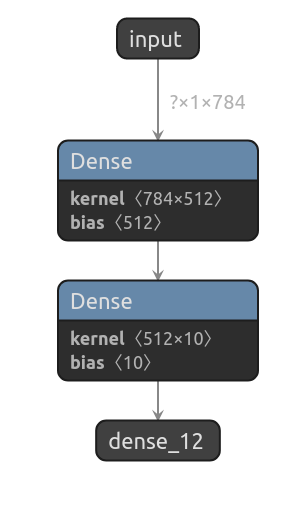
\includegraphics[scale=0.35]{tex/inc/img/keras.png}
        \caption{Keras сеть}
    \end{center}
\end{figure}

\subsubsection{Circle модель}

Поскольку добавленный инструмент работает только с circle моделями, необходимо сконвертировать обученную модель в необходимый формат. Для этого можно воспользоваться уже имеющимся в ONE инструментом tf2circleV2. На рис. 2.3 показан граф этой модели.

\begin{figure}[H]
    \begin{center}
        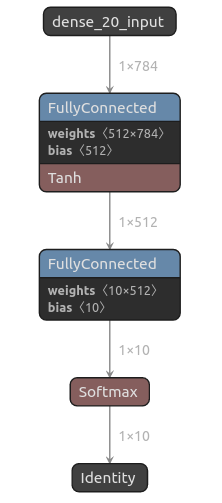
\includegraphics[scale=0.5]{tex/inc/img/circle.png}
        \caption{Circle сеть}
    \end{center}
\end{figure}

\subsubsection{Квантизованная модель}

Для обучения параметров квантизации следует воспользоваться добавленным в этой работе инструментом, однако перед этим необходимо подготовить выборку, которая будет прогоняться через сеть для получения распределения входных параметров. lquantizer позволяет работать с данными в формате hdf5, поэтому перед этим обучающий и валидационный датасеты были преобразованы в этот формат.

Воспользоваться новым инструментом возможно через bash терминал linux при помощи команды с листинга 2.6.

\begin{lstlisting}[language=bash, caption={Пример запуска квантизатора}]
./lquantizer --input_model model.circle  --output_model answer.circle \
             --input_data train.hdf5 --encode_bits 3
\end{lstlisting}

После некоторого ожидания lquantizer создает новый файл с квантизованной моделью, структура которой отражена на рис. 2.4.

\begin{figure}[H]
    \begin{center}
        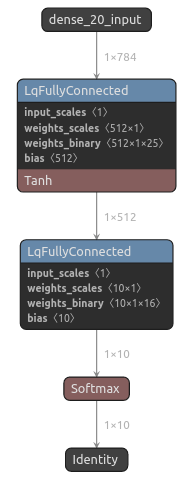
\includegraphics[scale=0.5]{tex/inc/img/lqcircle.png}
        \caption{Квантизованная сеть}
    \end{center}
\end{figure}

% -msse4.2
\subsection{Результаты}

При сравнении моделей основными метриками являются объем памяти, занимаемый сетью, средняя скорость её работы и точность на валидационной выборке, на которой не обучалась ни одна из них. 

\subsubsection{Оценка занимаемой памяти}

Для того, чтобы оценить объем памяти, занимаемый моделью, достаточно посмотреть на вес файла, в котором она хранится. Результаты представлены в таблице 2.1.

\begin{table}[H]
\caption{Занимаемая память исходной и квантизованных моделей}
\begin{center}
\begin{tabular}{|c|c|c|c|c|}
\hline
 -  & fp32 & int3 & int2 & int1 \\
\hline
Объём & 2.1 Mb & 218.3 Kb & 147.2 Kb & 76.2 Kb \\
\hline
\end{tabular}
\end{center}
\end{table}

\subsubsection{Оценка качества обучения}

Чтобы оценить работу алгоритма обучения, следует рассмотреть насколько удачно обучаются уровни квантизации для параметров нейронных слоёв. Гистограмма значений весов и уровни квантизации для случайного нейрона в первом слое рассматриваемой модели отображены на рис. 2.5.

\begin{figure}[H]
    \begin{center}
        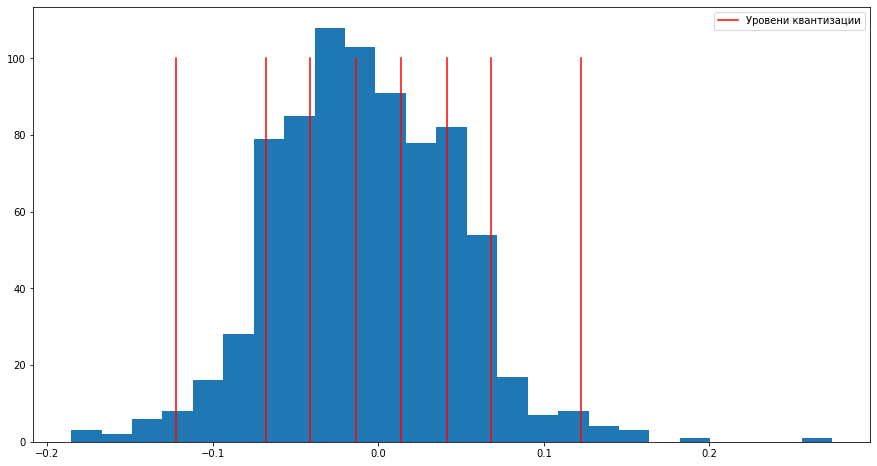
\includegraphics[scale=0.5]{tex/inc/img/firstneuro.png}
        \caption{Распределение весов и уровней квантизации в нейроне}
    \end{center}
\end{figure}


Стоит отметить, что уровни квантизации плотнее расположены к тем значениям весов, которые встречаются в нейроне наиболее часто.

Поскольку датасет, на котором обучалась модель, является сбалансированным, для оценки точности модели можно воспользоваться метрикой Accuracy по формуле (2.1), где $True$ означает количество правильных ответов сети, а $Count$ - количество записей в датасете.

\begin{equation}
Accuracy = \frac{True}{Count}
\end{equation}

Для того, чтобы получать ответы оцениваемых нейронных сетей на валидационной выборке, была написана несложная программа,  которая вызывает в себе luci\_interpreter на данных из hdf5 файла и замеряет время работы каждого вызова. После чего, при помощи скрипта на языке Python подсчитывается значение метрики Accuracy. Результаты проведенных замеров приведены в таблице 2.2.

\begin{table}[H]
\caption{Показатели точности исходной и квантизованных моделей}
\begin{center}
\begin{tabular}{|c|c|c|c|c|}
\hline
 -  & fp32 & int3 & int2 & int1 \\
\hline
Accuracy & 97.19 \% & 95.59 \% & 88.86 \% & 75.11 \% \\
\hline
\end{tabular}
\end{center}
\end{table}

\subsubsection{Оценка производительности}

Оценка производительности производится путем сравнения среднего времени работы нейронных сетей на наборе входных данных. Для этого в программе, реализованной для оценки точности, присутствует опция замера времени работы сети для каждого из входных векторов.

Характеристики ЭВМ, на котором производился запуск:
\begin{itemize}
    \item Операционная система: Ubuntu 18.04.5 LTS
    \item Количество ОЗУ: 16Гб
    \item Процессор: Intel Core i7-8550U CPU @ 1.80GHz × 8 (имеется поддержка SSE 4.2)
    \item Версия компилятора: gcc 7.5.0
\end{itemize}

Чтобы оценить насколько возрастает скорость работы квантизованных сетей при использовании процессорной инструкции POPCNT из набора SSE 4.2, были проведены замеры при стандартной сборке luci\_interpreter и с опцией компилятора -msse4.2. Результаты замеров отображены в таблице 2.3.

\begin{table}[H]
\caption{Производительность исходной и квантизованных моделей}
\begin{center}
\begin{tabular}{|c|c|c|c|c|}
\hline
 -  & fp32 & int3 & int2 & int1 \\
\hline
x86 & \textbf{584.829 мкс} & \textbf{510.210 мкс} & \textbf{256.711 мкс} & \textbf{82.0352 мкс} \\
\hline
SSE 4.2 & \textbf{583.931 мкс} & \textbf{152.743 мкс} & \textbf{84.7845 мкс} & \textbf{44.7829 мкс} \\
\hline
\end{tabular}
\end{center}
\end{table}


\backmatter %% Здесь заканчивается нумерованная часть документа и начинаются ссылки и
            %% заключение

\Conclusion % заключение к отчёту

\begin{center}
ЗАКЛЮЧЕНИЕ
\end{center}

В результате выполнения ВКР были достигнуты следующие цели:
\begin{itemize}
    \item Изучены существующие алгоритмы квантизации и проанализированы их преимущества и недостатки.
    \item Выбран фреймворк, в рамках которого была реализована предлагаемая в этой работе функциональность.
    \item Подобрана схема хранения и использования квантизованных значений и параметров.
    \item Добавлен нейронный слой с квантизованными параметрами.
    \item Реализовано вычислительное ядро для работы слоя.
    \item Написан инструмент квантизации предобученных сетей.
    \item Проанализированы показатели полученных моделей.
\end{itemize}


Реализованное в данной работе программное обеспечение может стать решением проблемы ограниченности ресурсов на микроконтроллерах и прочих недорогих устройствах для тех разработчиков, чьи продукты тесно связаны с нейронными сетями. 

Созданный инструмент планируется расширить возможностью квантизации сверточных слоев с соответствующей поддержкой в интерпретаторе и графовых представлениях фреймворка. 

\Biblio
\begin{center}
СПИСОК ИСПОЛЬЗОВАННЫХ ИСТОЧНИКОВ
\end{center}


\bibliographystyle{gost780u}
\begin{thebibliography}{9}
    \bibitem{lq} Dongqing Zhang, Jiaolong Yang, Dongqiangzi Ye, Gang Hua. (2018). LQ-Nets: Learned Quantization for Highly Accurate and Compact Deep Neural Networks. Proceedings of the European Conference on Computer
Vision (ECCV), 2018, pp. 365-382

    \bibitem{quantization}
    Raghuraman Krishnamoorthi. (2018). Quantizing deep convolutional networks for efficient inference: A whitepaper. arXiv:1806.08342.

    \bibitem{bqgemm} Yongkweon Jeon, Baeseong Park, Se Jung Kwon, Byeongwook Kim, Jeongin Yun, and Dongsoo Lee. (2020). BiqGEMM: matrix multiplication with lookup table for binary-coding-based quantized DNN's. arXiv:2005.09904.
    
    \bibitem{bench} Prateeth Nayak, David Zhang, Sek Chai. (2019). Bit Efficient Quantization for Deep Neural Networks arXiv:1910.04877.
    
    \bibitem{discret} А. Ю. Морозов, Д. Л. Ревизников, К. К. Абгарян. (2019). Вопросы реализации нейросетевых алгоритмов на мемристорных кроссбарах. Известия высших учебных заведений. Материалы электронной техники. 2019. Т. 22, № 4. C. 272—278.
    
    \bibitem{conv} Shujian Yu, Kristoffer Wickstrøm, Robert Jenssen, Jose C. Principe. (2020). Understanding Convolutional Neural Networks with Information Theory: An Initial Exploration. arXiv:1804.06537
    
    \bibitem{im2col} Sangkug Lym, Donghyuk Lee, Mike O’Connor, Niladrish Chatterjee, Mattan Erez. DeLTA: GPU Performance Model for Deep Learning Applications with In-depth Memory System Traffic Analysis. arXiv:1904.01691.
    
    \bibitem{gru} Rahul Dey, Fathi M. Salem. (2017). Gate-Variants of Gated Recurrent Unit (GRU) Neural Networks. arXiv:1701.05923.
    
    \bibitem{memristor} M.S. Tarkov, M.I. Osipov. (2016). The memristor crossbar-based WTA neural network. Bull. Nov. Comp. Center, Comp. Science, 39 (2016), 69–75.
    
    \bibitem{lstm} Ralf C. Staudemeyer, Eric Rothstein Morris. (2019). Understanding LSTM: a tutorial into Long Short-Term Memory Recurrent Neural Networks. arXiv:1909.09586.
    
    \bibitem{rnn} Ф.М. Гафаров, А.Ф. Галимьянов. (2018). Искусственные нейронные сети и их приложения. Издательство Казанского университета, 2018.
    
    \bibitem{intel} Intel. (2007). Intel SSE4 Programming Reference. 2006-2007 Intel Corporation.
    
    \bibitem{neon} Andrey Kamaev. (2012). Arm NEON SIMD. URL: http://www.itlab.unn.ru/file.php?id=731
    
\end{thebibliography}

\appendix   % Тут идут приложения

% \chapter{Первое Приложение}

\end{document}
